\documentclass[12pt]{ociamthesis}  % default square logo 
%\documentclass[12pt,beltcrest]{ociamthesis} % use old belt crest logo
%\documentclass[12pt,shieldcrest]{ociamthesis} % use older shield crest logo

%load any additional packages
\usepackage{amssymb}
\usepackage{listings}

\usepackage{color}
 
\definecolor{codegreen}{rgb}{0,0.6,0}
\definecolor{codegray}{rgb}{0.5,0.5,0.5}
\definecolor{codepurple}{rgb}{0.58,0,0.82}
\definecolor{backcolour}{rgb}{0.95,0.95,0.92}
 
\lstdefinestyle{mystyle}{
    backgroundcolor=\color{backcolour},   
    commentstyle=\color{codegreen},
    keywordstyle=\color{magenta},
    numberstyle=\tiny\color{codegray},
    stringstyle=\color{codepurple},
    basicstyle=\footnotesize,
    breakatwhitespace=false,         
    breaklines=true,                 
    captionpos=b,                    
    keepspaces=true,                 
    numbers=left,                    
    numbersep=5pt,                  
    showspaces=false,                
    showstringspaces=false,
    showtabs=false,                  
    tabsize=2,
    language=python
}
 
\lstset{style=mystyle}
%input macros (i.e. write your own macros file called mymacros.tex 
%and uncomment the next line)
%\include{mymacros}

\title{Tugas \\[1ex]     %your thesis title,
        Kecerdasan Buatan}   %note \\[1ex] is a line break in the title

\author{Faisal Abdullah}             %your name
\college{1194014\\[5ex]
Applied Bachelor of Informatics Engineering}  %your college

%\renewcommand{\submittedtext}{change the default text here if needed}
\degree{Politeknik Pos Indonesia}     %the degree
\degreedate{Bandung 2022}         %the degree date

%end the preamble and start the document
\begin{document}

%this baselineskip gives sufficient line spacing for an examiner to easily
%markup the thesis with comments
\baselineskip=18pt plus1pt

%set the number of sectioning levels that get number and appear in the contents
\setcounter{secnumdepth}{3}
\setcounter{tocdepth}{3}


\maketitle                  % create a title page from the preamble info
\include{section/dedication}        % include a dedication.tex file
\include{section/acknowlegements}   % include an acknowledgements.tex file
\include{section/abstract}          % include the abstract

\begin{romanpages}          % start roman page numbering
\tableofcontents            % generate and include a table of contents
\listoffigures              % generate and include a list of figures
\end{romanpages}            % end roman page numbering

%now include the files of latex for each of the chapters etc
\chapter{Mengenal Kecerdasan Buatan dan Scikit-Learn}

\section{Teori}
Praktek teori penunjang yang dikerjakan :
\begin{enumerate}
\item
Definisi, Sejarah dan perkembangan Kecerdasan Buatan \textit{Artifical Intelligence}. \textit{Artifical Intelligence} adalah  ilmu yang ada pada bidang komputer yang memungkinkan  suatu sistem  untuk menyelesaikan permasalahan.\\
Pada akhir tahun 1955 AI pertama muncul berkat Newell dan Simon dengan adanya perkembangan perkembangan \textit{The Logic Theorist} .Pada 1956, istilah AI pertama kali diciptakan di Darmouth College ketika menyelengarakan konferensi dengan nama \textit{The Dartmouth summer research project on artificial intelligence}. konferensi tersebut diselengarakan untuk memancing para ahli.

\item
Definisi supervised learning, klasifikasi, regresi dan unsupervised learning. Data set, training set dan testing set.
\begin{itemize}

	\item Supervised Learning
    \par
    \textit{Supervised Learning} sebuah pembelajaran yang ditentukan berdasarkan penggunaan traning set yang berlabel.

    \item Klasifikasi
    \par
    Klasifikasi adalah mengidentifikasi suatu data menjadi sebuah bagian dari kelas berdasarkan label.

	\item Regresi
	\par 
	Regresi adalah mendefinisikan relasi antara dua variable maupun lebih seperti variable terikat dan variabel bebas untuk melihat selisih nilai prediksi dengan nilai real.

    \item Data set, Training set dan Testing set
    \par
    Data set adalah kumpulan data. Kemudian training set adalah  data set yang berfungsi melatih suatu algoritma untuk mencapai suatu tujuan, dan testing set yaitu data set yang digunakan untuk mengetahui akurasi dari algoritma yang sudah di latih sebelumnya.

	\item Unsupervised Learning
	\par
	\textit{Unsupervised Learning} sebuah pembelajaran yang ditentukan berdasarkan penggunaan traning set yang tidak berlabel. 

\end{itemize}
\end{enumerate}

\section{Instalasi}
\begin{enumerate}
\item
Instalasi library scikit dari anaconda, mencoba kompilasi dan uji coba ambil contoh kode dan lihat variabel explorer.\\
gunakan "pip install -U scikit-learn"\\
https://youtu.be/xvX7Pye2Npw
\begin{figure}[!htbp]
    \centering
    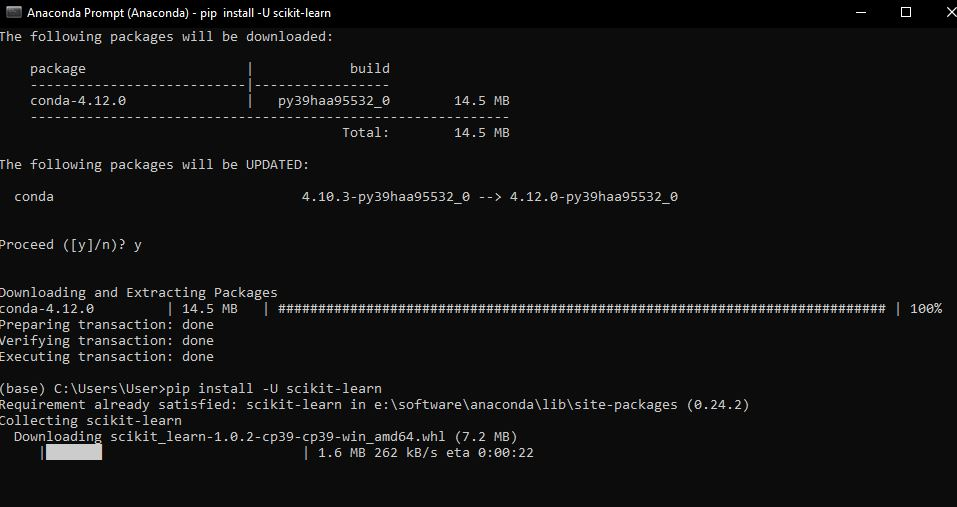
\includegraphics[scale=0.4]{figures/1.JPG}
	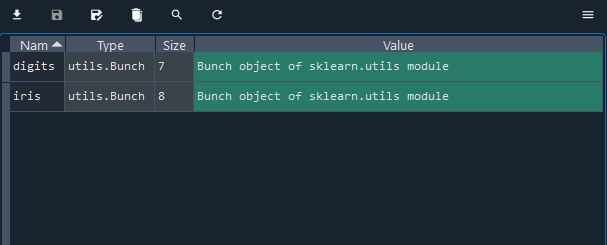
\includegraphics[scale=0.4]{figures/1.1.JPG}
    \end{figure}

\item
Mencoba Loading an example dataset, menjelaskan maksud dari tulisan tersebut dan mengartikan per baris
\begin{figure}[!htbp]
    \centering
    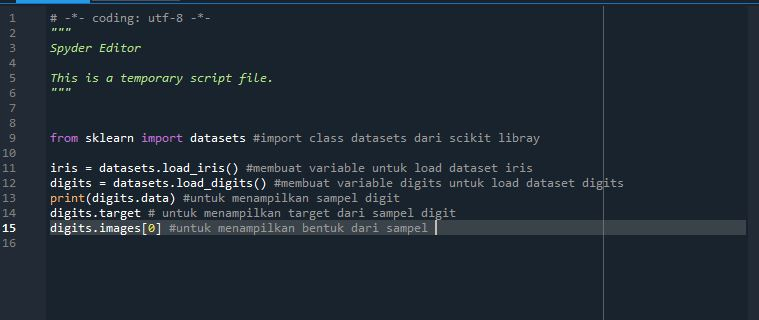
\includegraphics[scale=0.4]{figures/3.JPG}
    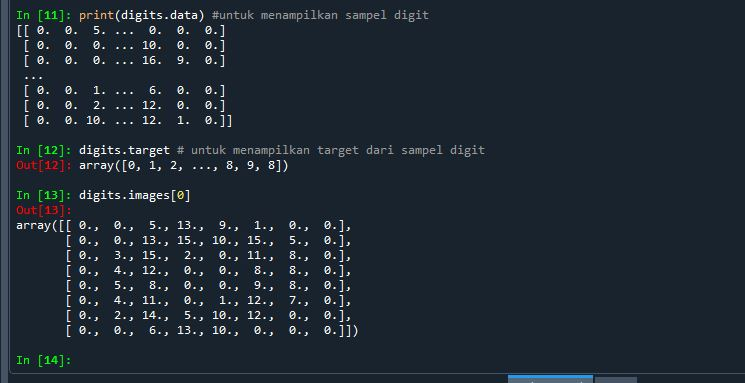
\includegraphics[scale=0.3]{figures/3.1.JPG}
    \end{figure}

\newpage
\item
Mencoba Learning and predicting, menjelaskan maksud dari tulisan tersebut dan mengartikan per baris
\begin{figure}[!htbp]
    \centering
    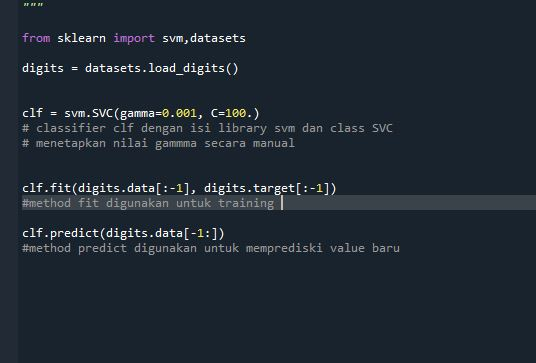
\includegraphics[scale=0.4]{figures/4.JPG}
    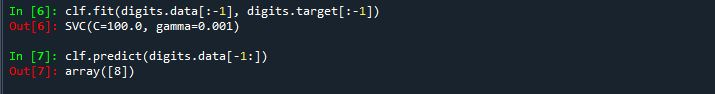
\includegraphics[scale=0.4]{figures/4.1.JPG}
    \end{figure}


\item
Mencoba Model persistence, menjelaskan maksud dari tulisan tersebut dan mengartikan per baris. menggunakan 2 cara yaitu menggunakan pickle atau menggunakan joblib
\begin{figure}[!htbp]
    \centering
    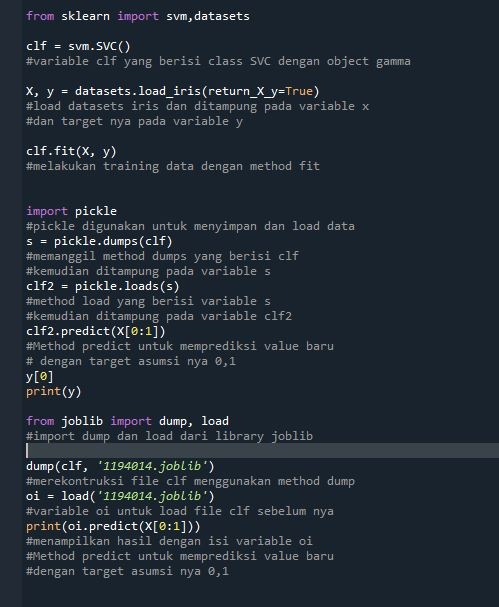
\includegraphics[scale=0.4]{figures/5.JPG}\\
    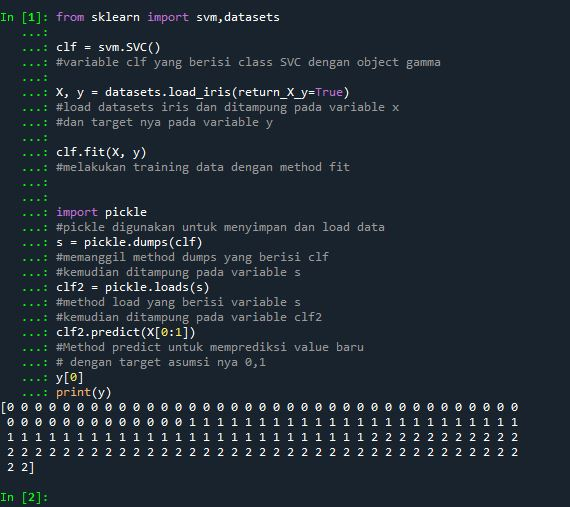
\includegraphics[scale=0.3]{figures/5.1.JPG}
    \end{figure}

\newpage
\begin{figure}[!htbp]
    \centering
    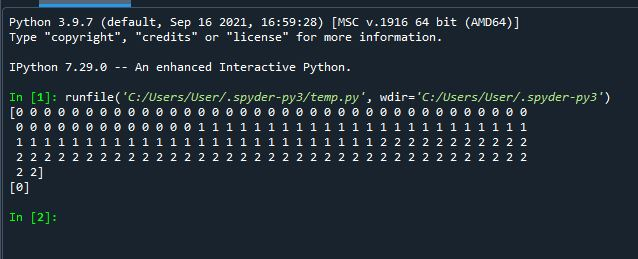
\includegraphics[scale=0.3]{figures/5.2.JPG}
    \end{figure}


\item 
Mencoba Conventions, menjelaskan maksud dari tulisan tersebut dan mengartikan per baris 
\begin{lstlisting}[language=Python]
import numpy as np  #library
from sklearn import random_projection, svm, datasets 
from sklearn.datasets import load_iris
from sklearn.multiclass import OneVsRestClassifier
from sklearn.preprocessing import LabelBinarizer
from sklearn.preprocessing import MultiLabelBinarizer
from sklearn.svm import SVC

iris = datasets.load_iris()


#Type Casting
rng = np.random.RandomState(0) 
X = rng.rand(10, 2000) 
X = np.array(X, dtype='float32')
print(X.dtype)

transformer = random_projection.GaussianRandomProjection()
X = transformer.fit_transform(X)
print(X.dtype)

clf = svm.SVC()
clf.fit(iris.data, iris.target)
print(clf.fit(iris.data, iris.target))

list(clf.predict(iris.data[:3]))

print((clf.predict(iris.data[:3])))

clf.fit(iris.data, iris.target_names[iris.target])
print(clf.fit(iris.data, iris.target_names[iris.target]))

list(clf.predict(iris.data[:3]))
print(list(clf.predict(iris.data[:3])))

#refitting and updating paramater
X, y = load_iris(return_X_y=True)
clf = svm.SVC()

clf.set_params(kernel='linear').fit(X, y)
print(clf.set_params(kernel='linear').fit(X, y))

clf.predict(X[:5])
print(clf.predict(X[:5]))

#Multiclass vs multilabel fitting
X = [[1, 2], [2, 4], [4, 5], [3, 2], [3, 1]]
y = [0, 0, 1, 1, 2]

classif = OneVsRestClassifier(estimator=SVC(random_state=0))
classif.fit(X, y).predict(X)
print(classif.fit(X, y).predict(X))

y = LabelBinarizer().fit_transform(y)
classif.fit(X, y).predict(X)
print(classif.fit(X, y).predict(X))

y = y = [[0, 1], [0, 2], [1, 3], [0, 2, 3], [2, 4]]
y = MultiLabelBinarizer().fit_transform(y)
print(classif.fit(X, y).predict(X))
\end{lstlisting}
\end{enumerate}



\section{Penanganan Error}
Dari percobaan yang dilakukan di atas, apabila mendapatkan error maka:

\begin{enumerate}
	\item
	skrinsut error\
    \begin{figure}[!htbp]
        \centering
        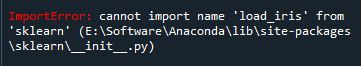
\includegraphics[scale=0.5]{figures/6.JPG}
        \end{figure}

	\item
Tuliskan kode eror dan jenis errornya\
    \begin{enumerate}
        \item Import Error terjadi ketika suatu modul tidak ditemukan
    \end{enumerate}

	\item
Solusi pemecahan masalah error tersebut\
\begin{enumerate}
    \item Pastikan memasukan nama modul yang tepat \
    \begin{figure}[!htbp]
        \centering
        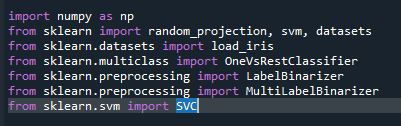
\includegraphics[scale=0.7]{figures/7.JPG}
        \end{figure}
    
\end{enumerate}

\end{enumerate}


% \chapter{Membangun Model Prediksi}

% Untuk pratikum saati ini menggunakan buku \textit{Python Artificial Intelligence Projects for Beginners}\cite{eckroth2018python}. Dengan praktek menggunakan python 3 dan editor anaconda dan library python scikit-learn.
% Dataset ada di https://github.com/PacktPublishing/Python-Artificial-Intelligence-Projects-for-Beginners .
% Tujuan pembelajaran pada pertemuan pertama antara lain:
% \begin{enumerate}
% \item
% Mengerti implementasi klasifikasi
% \item
% Memahami data set, training dan testing data
% \item
% Memahami Decission tree.
% \item
% Memahami information gain dan entropi.
% \end{enumerate}
% Tugas dengan cara dikumpulkan dengan pull request ke github dengan menggunakan latex pada repo yang dibuat oleh asisten riset. Kode program menggunakan input listing ditaruh di folder src ekstensi .py dan dipanggil ke latex dengan input listings. Tulisan dan kode tidak boleh plagiat, menggunakan bahasa indonesia yang sesuai dengan gaya bahasa buku teks.

\section{Teori}
Praktek teori penunjang yang dikerjakan(nilai 5 per nomor, untuk hari pertama) :
\begin{enumerate}
\item
Jelaskan apa itu binary classification dilengkapi ilustrasi gambar sendiri\\
Binary classification adalah proses mengklasifikasi yang ouputnya dibagi menjadi 2 kelas 

\item
Jelaskan apa itu supervised learning dan unsupervised learning dan clustering dengan ilustrasi gambar sendiri.
\par
    \textit{Supervised Learning} sebuah pembelajaran yang ditentukan berdasarkan penggunaan traning set yang berlabel.
\par
    \textit{Unsupervised Learning} sebuah pembelajaran yang ditentukan berdasarkan penggunaan traning set yang tidak berlabel. 

\item
Jelaskan apa itu evaluasi dan akurasi dari buku dan disertai ilustrasi contoh dengan gambar sendiri
\par
    Evaluasi adalah tentang mengukur sebarapa baik nilai performa dari suatu model. Dan akurasi adalah tigkat ketepatan yang benar dari suatu model.
    
\item
Jelaskan bagaimana cara membuat dan membaca confusion matrix, buat confusion matrix buatan sendiri.\\
Cara membuat dan membaca confusion matrix :
\begin{enumerate}
    \item Tentukan studi kasus nya
    \item Buat ke dalam Decision Tree
    \item Siapkan data testing 
    \item Kemudian cari value dari variabel misal nya a,b,c,d
    \item Dan cari value dari recall, precision, accuracy dan juga error state
\end{enumerate}

\item
Jelaskan bagaimana K-fold cross validation bekerja dengan gambar ilustrasi contoh buatan sendiri.
Cara kerja dari K-fold cross validation :
\begin{enumerate}
    \item Total instace dibagi menjadi n bagian
    \item Fold pertama merupakan bagian pertama yang menjadi Testing data dan sisanya menjadi training data
    \item Hitung akurasinya dengan menggunakan persamaan
    \item Fold ke dua merupakan bagian kedua yang menjadi testing data dan sisanya mendjadi training data
    \item Hitung lagi akurasi nya dan juga seterus nya pada fold yang terakhir
    \item Dan terakhir adalah hitung rata-rata akurasi nya
\end{enumerate}
\begin{figure}[!htbp]
    \centering
    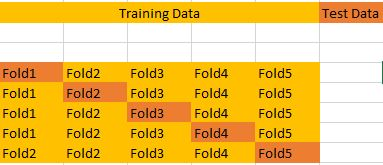
\includegraphics[scale=0.5]{figures/K-fold.JPG}
	\caption{Ilutrasi K-fold cross validation}
\end{figure}


\item
Jelaskan apa itu decision tree dengan gambar ilustrasi contoh buatan sendiri.\\
Decision Tree adalah suatu metode yang digunakan untuk mengambil keputusan


\item
Jelaskan apa itu information gain dan entropi dengan gambar ilustrasi buatan sendiri.\\
information gain adalah kumpulan informasi yang diperolah dari variable acak. Dan Entropi adalah tingkat keacakan pada informasi yang sedang diproses.\\



\end{enumerate}

\section{scikit-learn}
Dataset ambil di https://github.com/PacktPublishing/Python-Artificial-Intelligence-Projects-for-Beginners folder Chapter01.
Tugas anda adalah, dataset ganti menggunakan \textbf{student-mat.csv} dan mengganti semua nama variabel dari kode di bawah ini dengan nama-nama makanan (NPM mod 3=0), kota (NPM mod 3=1), buah (NPM mod 3=2), . Jalankan satu per satu kode tersebut di spyder dengan menggunakan textit{Run current cell}. Kemudian Jelaskan dengan menggunakan bahasa yang mudah dimengerti dan bebas plagiat dan wajib skrinsut dari komputer sendiri masing masing nomor di bawah ini(nilai 5 masing masing pada hari kedua).

\begin{enumerate}

\item load dataset student-mat.csv
\begin{figure}[!htbp]
    \centering
    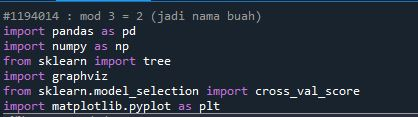
\includegraphics[scale=0.5]{figures/importchap2.JPG}
	\caption{Import}
    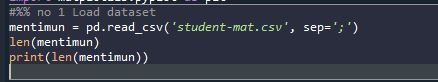
\includegraphics[scale=0.5]{figures/Chap2-1.JPG}
	\caption{Source Code Task 1}
    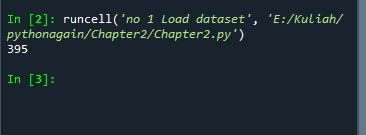
\includegraphics[scale=0.5]{figures/Chap2-1.1.JPG}
	\caption{Hasil Task}
\end{figure}

\newpage
\item generate binary label
\begin{figure}[!htbp]
    \centering
    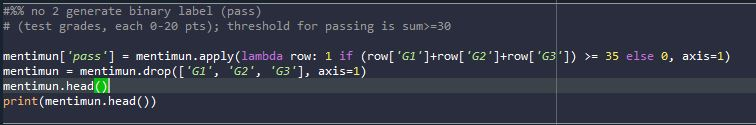
\includegraphics[scale=0.4]{figures/Chap2-2.JPG}
	\caption{Source Code Task 2}
    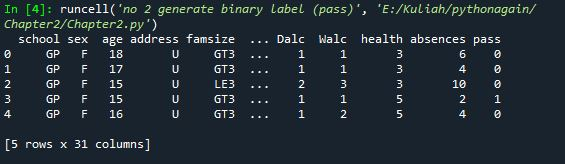
\includegraphics[scale=0.5]{figures/Chap2-2.1.JPG}
	\caption{Hasil Task 2}
\end{figure}

\item use one-hot encoding on categorical columns
\begin{figure}[!htbp]
    \centering
    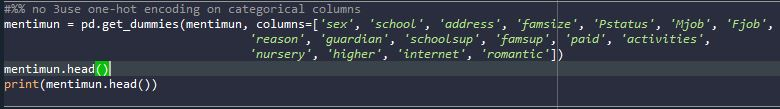
\includegraphics[scale=0.4]{figures/Chap3-1.JPG}
	\caption{Source Code Task 3}
    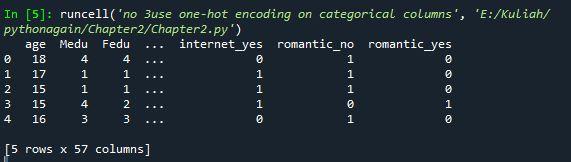
\includegraphics[scale=0.5]{figures/Chap3-1.1.JPG}
	\caption{Hasil Task 3}
\end{figure}

\item shuffle rows
\begin{figure}[!htbp]
    \centering
    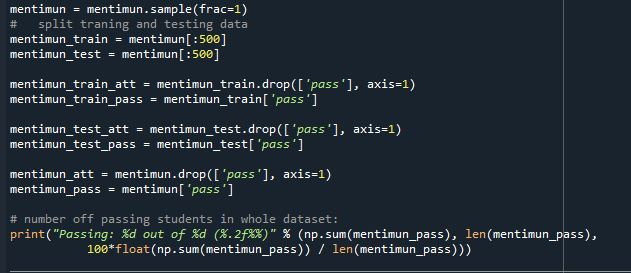
\includegraphics[scale=0.4]{figures/Chap4-1.JPG}
	\caption{Source Code Task 4}
	\newpage
    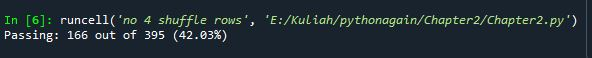
\includegraphics[scale=0.5]{figures/Chap4-1.1.JPG}
	\caption{Hasil Task 4}
\end{figure}

\newpage
\item fit a decision tree
\begin{figure}[!htbp]
    \centering
    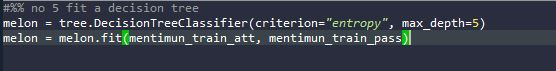
\includegraphics[scale=0.5]{figures/Chap5-1.JPG}
	\caption{Source Code Task 5}
	
    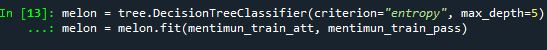
\includegraphics[scale=0.5]{figures/Chap5-1.1.JPG}
	\caption{Hasil Task 5}
\end{figure}


\item visualize tree
\begin{figure}[!htbp]
    \centering
    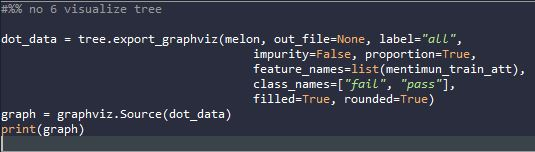
\includegraphics[scale=0.5]{figures/Chap6-1.JPG}
	\caption{Source Code Task 6}
    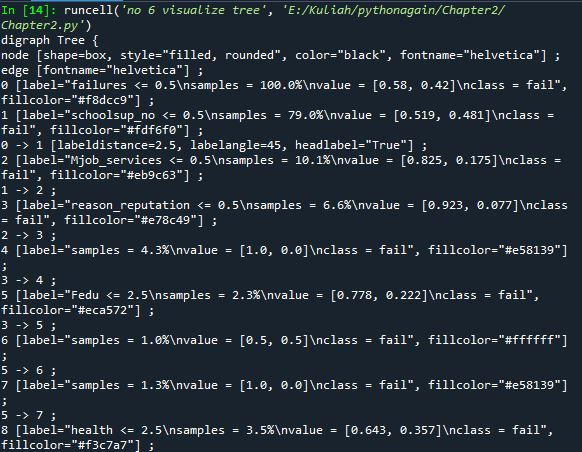
\includegraphics[scale=0.5]{figures/Chap6-1.1.JPG}
	\caption{Hasil Task 6}
\end{figure}

\newpage
\item save tree
\begin{figure}[!htbp]
    \centering
    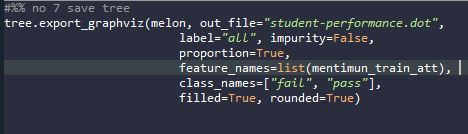
\includegraphics[scale=0.5]{figures/Chap7-1.JPG}
	\caption{Source Code Task 7}
    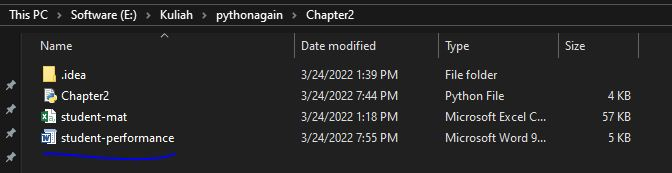
\includegraphics[scale=0.5]{figures/Chap7-1.1.JPG}
	\caption{Hasil Task 7}
    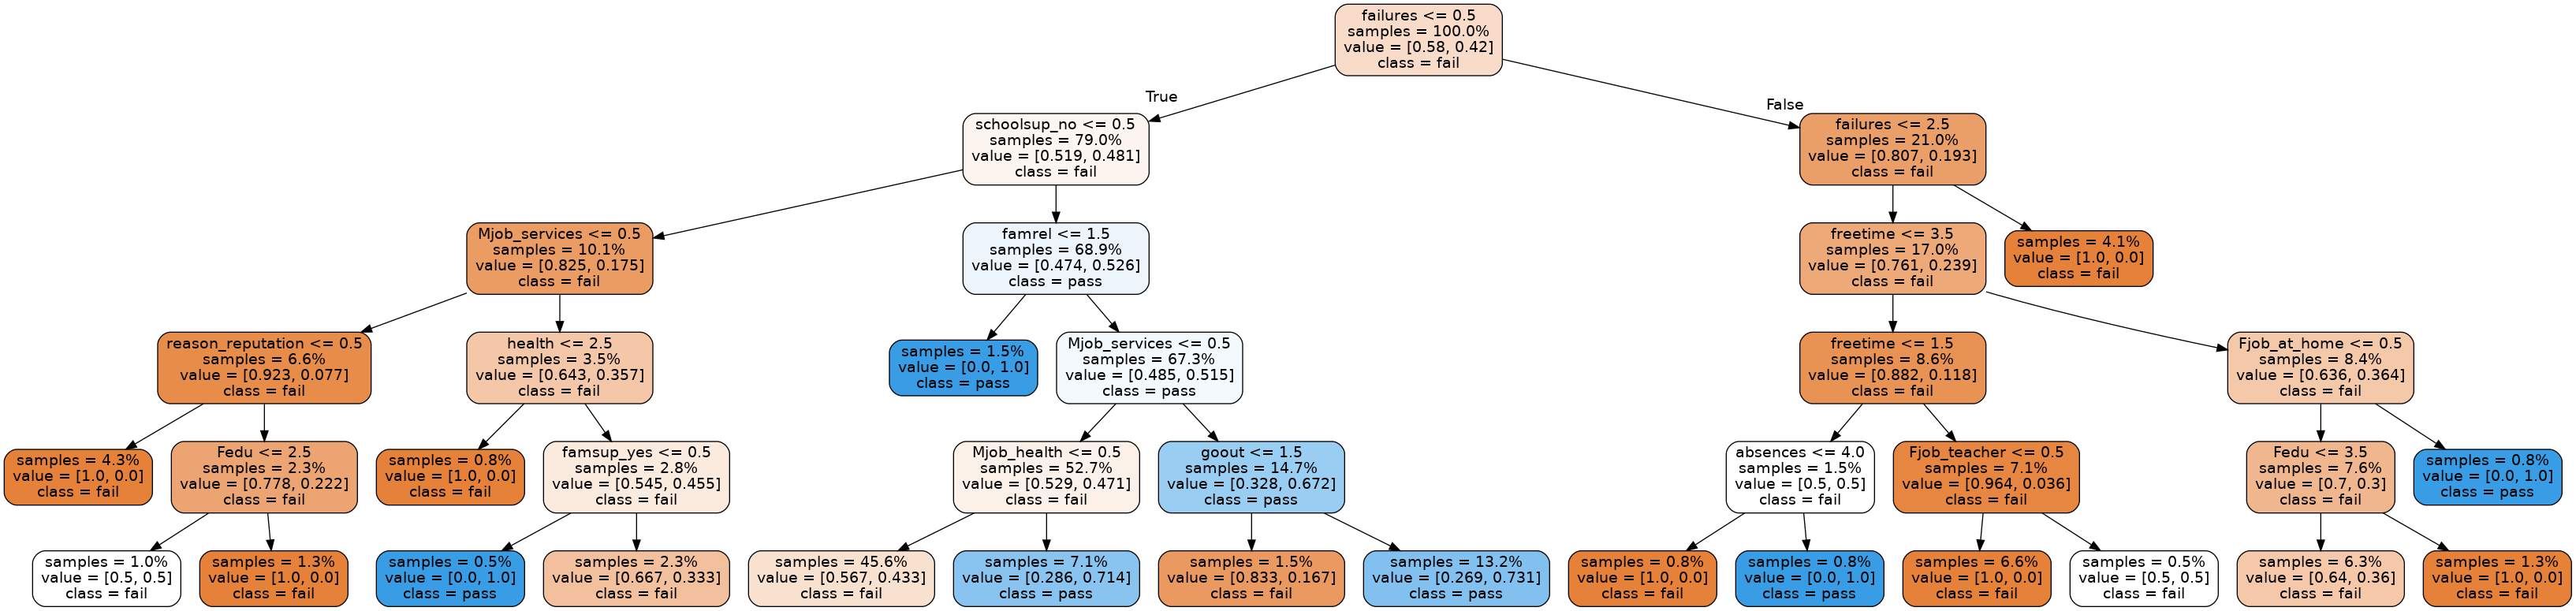
\includegraphics[scale=0.1]{figures/student-performance.png}
	\caption{Hasil Task 7}
\end{figure}

\item task 8
\begin{figure}[!htbp]
    \centering
    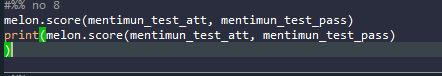
\includegraphics[scale=0.5]{figures/Chap8-1.JPG}
	\caption{Source Code Task 8}
    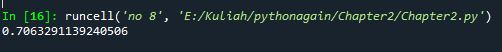
\includegraphics[scale=0.5]{figures/Chap8-1.1.JPG}
	\caption{Hasil Task 8}
\end{figure}


\item task 9
\begin{figure}[!htbp]
    \centering
    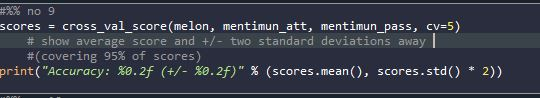
\includegraphics[scale=0.5]{figures/Chap9-1.JPG}
	\caption{Source Code Task 9}
    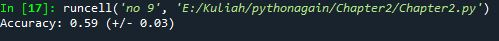
\includegraphics[scale=0.5]{figures/Chap9-1.1.JPG}
	\caption{Hasil Task 9}
\end{figure}

\newpage
\item task 10
\begin{figure}[!htbp]
    \centering
    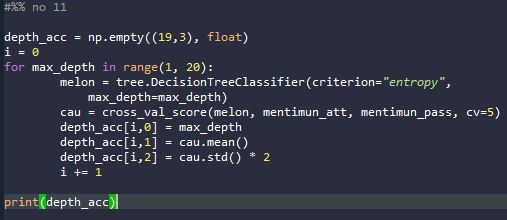
\includegraphics[scale=0.5]{figures/Chap11-1.JPG}
	\caption{Source Code Task 10}
    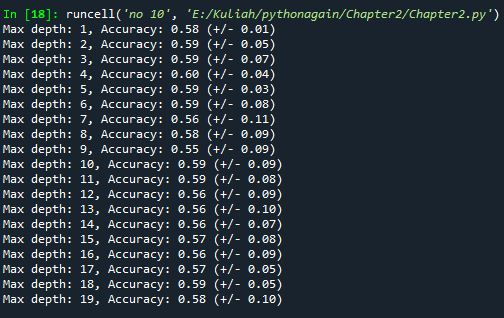
\includegraphics[scale=0.5]{figures/Chap10-1.1.JPG}
	\caption{Hasil Task 10}
\end{figure}


\item task 11
\begin{figure}[!htbp]
    \centering
    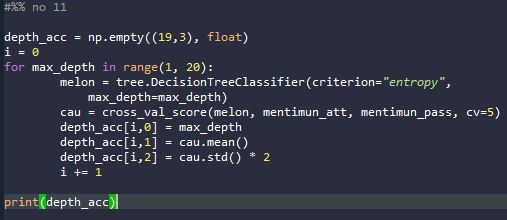
\includegraphics[scale=0.5]{figures/Chap11-1.JPG}
	\caption{Source Code Task 11}
    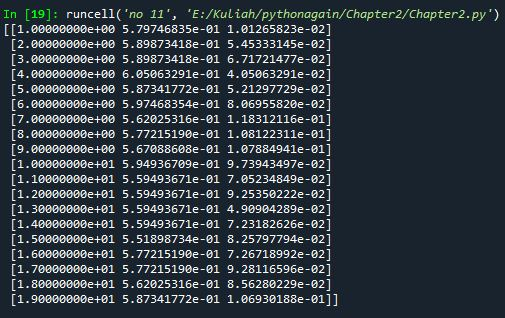
\includegraphics[scale=0.5]{figures/Chap11-1.1.JPG}
	\caption{Hasil Task 11}
\end{figure}

\newpage
\item task 12
\begin{figure}[!htbp]
    \centering
    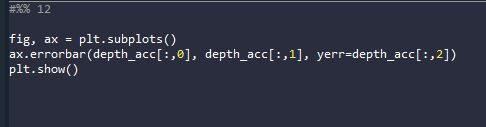
\includegraphics[scale=0.5]{figures/Chap12-1.JPG}
	\caption{Source Code Task 12}
    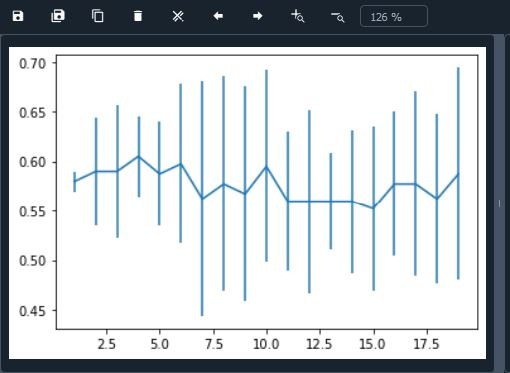
\includegraphics[scale=0.5]{figures/Chap12-1.1.JPG}
	\caption{Hasil Task 12}
\end{figure}

\end{enumerate}


\section{Penanganan Error}
Dari percobaan yang dilakukan di atas, error yang kita dapatkan di dokumentasikan dan di selesaikan(nilai 5 hari kedua):

\begin{enumerate}
	\item
skrinsut error
	\item
Tuliskan kode eror dan jenis errornya
	\item
Solusi pemecahan masalah error tersebut

\end{enumerate}


% \chapter{Prediksi dengan Random Forest}

Untuk pratikum saati ini menggunakan buku \textit{Python Artificial Intelligence Projects for Beginners}\cite{eckroth2018python}. Dengan praktek menggunakan python 3 dan editor anaconda dan library python scikit-learn.
Kode program ada di https://github.com/PacktPublishing/Python-Artificial-Intelligence-Projects-for-Beginners .
Tujuan pembelajaran pada pertemuan pertama antara lain:
\begin{enumerate}
\item
Mengerti implementasi klasifikasi dan teknik evaluasi
\item
Memprediksi spesies burung dengan random forest
\item
Memahami Confusion Matrix.
\end{enumerate}
Tugas dengan cara dikumpulkan dengan pull request ke github dengan menggunakan latex pada repo yang dibuat oleh asisten riset. Kode program menggunakan input listing ditaruh di folder src ekstensi .py dan dipanggil ke latex dengan input listings. Tulisan dan kode tidak boleh plagiat, menggunakan bahasa indonesia yang sesuai dengan gaya bahasa buku teks.

\section{Teori}
Random Forest adalah hasil voting dari beberapa decission tree yang masing-masing memegang atribut yang berbeda. Jadi setiap decission tree spesifik terhadap atribut tersebut yang merupakan bagian kecil dari keseluruhan atribut di data set. Hindari RF jika atribut terlalu sedikit untuk membentuk beberapa tree. Pada praktek kali ini mengggunakan dataset spesies burung yang diambil dari situs 
(http://www.vision.caltech.edu/visipedia/CUB-200-2011.html). Didalamnya terdapat 12.000 foto dari 200 spesies yang berbeda. Yang akan kita pakai untuk RF hanya atribut dari burunynya saja seperti ukuran, bentuk dan warna. Data tersebut diberi label secara manual oleh manusia dengan memanfaatkan jasa dari Amazon's Mechanical Turk.

\subsection{Random Forest}
Pertama dataset kita baca terlebih dahulu.
\begin{lstlisting}[caption=Membaca data file txt,label={lst:fungsisederhana}]
import pandas as pd

# some lines have too many fields (?), so skip bad lines
imgatt = pd.read_csv("data/CUB_200_2011/attributes/image_attribute_labels.txt",
                     sep='\s+', header=None, error_bad_lines=False, warn_bad_lines=False,
                     usecols=[0,1,2], names=['imgid', 'attid', 'present'])

\end{lstlisting}

Melihat sebagian data awal, dengan menggunakan listing \ref{lst:3.1}.

\begin{lstlisting}[caption=Melihat sebagian data awal,label={lst:3.1}]
imgatt.head()
\end{lstlisting}

Melihat jumlah data menggunakan listing \ref{lst:3.2}.
\begin{lstlisting}[caption=Mengetahui jumlah data,label={lst:3.2}]
imgatt.shape
\end{lstlisting}

Merubah atribut menjadi kolom dengan menggunakan pivot layaknya excel. lalu kita cek isinya dengan menggunakan perintah pada listing \ref{lst:3.3}.
\begin{lstlisting}[caption=Pivot dataset,label={lst:3.3}]
imgatt2 = imgatt.pivot(index='imgid', columns='attid', values='present')

imgatt2.head()
imgatt2.shape
\end{lstlisting}


Sekarang kita akan meload jawabannya yang berisi apakah burung itu termasuk dalam spesies yang mana. Dua kolomnya adalah imgid dan label. Dan melakukan pivot yang mana imgid menjadi index yang artinya unik perintahnya ada di listing \ref{lst:3.6}. Lalu kita cek kembali datanya. 
\begin{lstlisting}[caption=membaca dataset label file txt,label={lst:3.6}]
imglabels = pd.read_csv("data/CUB_200_2011/image_class_labels.txt", 
                        sep=' ', header=None, names=['imgid', 'label'])

imglabels = imglabels.set_index('imgid')


imglabels.head()
imglabels.shape
\end{lstlisting}

Karena isinya sama kita bisa melakukan join antara dua data. Sehingga kita akan mendapatkan data ciri dan data jawabannya atau labelnya sehingga bisa dikatekorikan supervised learning. maka perintah untuk menggabungkan kedua data dan kemudian kita melakukan pemisahan antara data set untuk training dan test dengan perintah di listing \ref{lst:3.7}.
\begin{lstlisting}[caption=Menggabungkan field dari dua file terpisah,label={lst:3.7}]
df = imgatt2.join(imglabels)
df = df.sample(frac=1)
\end{lstlisting}

Kemudian drop label yang didepan, dan gunakan label yang paling belakang yang baru di join dengan perintah listing \ref{lst:3.8}.
\begin{lstlisting}[caption=Memisahkan dan memilih label,label={lst:3.8}]
df_att = df.iloc[:, :312]
df_label = df.iloc[:, 312:]
\end{lstlisting}
Kita bisa mengecek isinya dengan perintah listing \ref{lst:3.9}.
\begin{lstlisting}[caption=Melihat isi masing masing data frame,label={lst:3.9}]
df_att.head()
df_label.head()
\end{lstlisting}

Kita bagi menjadi dua bagian, 8000 row pertama sebagai data training sisanya sebagai data testing dengan perintah listing \ref{lst:3.10}.
\begin{lstlisting}[caption=Pembagian data training dan test,label={lst:3.10}]
df_train_att = df_att[:8000]
df_train_label = df_label[:8000]
df_test_att = df_att[8000:]
df_test_label = df_label[8000:]

df_train_label = df_train_label['label']
df_test_label = df_test_label['label']
\end{lstlisting}

Kita panggil kelas RandomForestClassifier. max features diartikan sebagai berapa banyak kolom pada setiap tree dengan perintah listing \ref{lst:3.11}.
\begin{lstlisting}[caption=Instansiasi kelas Random Forest,label={lst:3.11}]
from sklearn.ensemble import RandomForestClassifier
clf = RandomForestClassifier(max_features=50, random_state=0, n_estimators=100)

\end{lstlisting}
Kemudian lakukan fit untuk membangun random forest yang sudah ditentukan dengan maksimum fitur sebanya 50 untuk perpohonnya dengan perintah listing \ref{lst:3.12}.

\begin{lstlisting}[caption=Fitting random forest dengan dataset training,label={lst:3.12}]
clf.fit(df_train_att, df_train_label)
\end{lstlisting}
Hasilnya bisa kita dapatkan dengan perintah predict dengan perintah listing \ref{lst:3.13}.
\begin{lstlisting}[caption=Melihat Hasil prediksi,label={lst:3.13}]
print(clf.predict(df_train_att.head()))
\end{lstlisting}

Untuk besaran akurasinya dengan perintah listing \ref{lst:3.14}
\begin{lstlisting}[caption=Score perolehan dari klasifikasi,label={lst:3.14}]
clf.score(df_test_att, df_test_label)
\end{lstlisting}

\subsection{Confusion Matrix}
Dari RF kita coba petakan ke dalam Confusion Matrix dan lihat hasilnya dengan perintah listing \ref{lst:3.15}.
\begin{lstlisting}[caption=Membuat Confusion Matrix,label={lst:3.15}]
from sklearn.metrics import confusion_matrix
pred_labels = clf.predict(df_test_att)
cm = confusion_matrix(df_test_label, pred_labels)

cm
\end{lstlisting}

Kemudian kita plot dengan perintah
\begin{lstlisting}[caption=Plotting Confusion Matrix,label={lst:3.16}]
import matplotlib.pyplot as plt
import itertools
def plot_confusion_matrix(cm, classes,
                          normalize=False,
                          title='Confusion matrix',
                          cmap=plt.cm.Blues):
    """
    This function prints and plots the confusion matrix.
    Normalization can be applied by setting `normalize=True`.
    """
    if normalize:
        cm = cm.astype('float') / cm.sum(axis=1)[:, np.newaxis]
        print("Normalized confusion matrix")
    else:
        print('Confusion matrix, without normalization')

    print(cm)

    plt.imshow(cm, interpolation='nearest', cmap=cmap)
    plt.title(title)
    #plt.colorbar()
    tick_marks = np.arange(len(classes))
    plt.xticks(tick_marks, classes, rotation=90)
    plt.yticks(tick_marks, classes)

    fmt = '.2f' if normalize else 'd'
    thresh = cm.max() / 2.
    #for i, j in itertools.product(range(cm.shape[0]), range(cm.shape[1])):
    #    plt.text(j, i, format(cm[i, j], fmt),
    #             horizontalalignment="center",
    #             color="white" if cm[i, j] > thresh else "black")

    plt.tight_layout()
    plt.ylabel('True label')
    plt.xlabel('Predicted label')

\end{lstlisting}

 Agar plot sumbunya sesuai dengan nama datanya maka kita set dengan perintah
\begin{lstlisting}[caption=Membaca file classes.txt,label={lst:3.17}]
birds = pd.read_csv("data/CUB_200_2011/classes.txt",
                    sep='\s+', header=None, usecols=[1], names=['birdname'])
birds = birds['birdname']
birds

\end{lstlisting}

Lalu kita plot
\begin{lstlisting}[caption=Plot hasil perubahan label,label={lst:3.18}]
import numpy as np
np.set_printoptions(precision=2)
plt.figure(figsize=(60,60), dpi=300)
plot_confusion_matrix(cm, classes=birds, normalize=True)
plt.show()
\end{lstlisting}



\subsection{Mencoba dengan metode Decission Tree dan SVM}
Kita coba menggunakan Decission tree 
\begin{lstlisting}[caption=Mencoba klasifikasi dengan decission tree dengan dataset yang sama,label={lst:3.19}]
from sklearn import tree
clftree = tree.DecisionTreeClassifier()
clftree.fit(df_train_att, df_train_label)
clftree.score(df_test_att, df_test_label)
\end{lstlisting}
Kita coba menggunakan SVM
\begin{lstlisting}[caption=Mencoba klasifikasi dengan SVM dengan dataset yang sama,label={lst:3.20}]
from sklearn import svm
clfsvm = svm.SVC()
clfsvm.fit(df_train_att, df_train_label)
clfsvm.score(df_test_att, df_test_label)
\end{lstlisting}

\subsection{Pengecekan Cross Validation}
Pengeceken Cross Validation untuk random forest
\begin{lstlisting}[caption=Hasil Cross Validation random forest,label={lst:3.21}]
from sklearn.model_selection import cross_val_score
scores = cross_val_score(clf, df_train_att, df_train_label, cv=5)
# show average score and +/- two standard deviations away (covering 95% of scores)
print("Accuracy: %0.2f (+/- %0.2f)" % (scores.mean(), scores.std() * 2))
\end{lstlisting}
untuk decission tree
\begin{lstlisting}[caption=Hasil Cross Validation Decission Tree,label={lst:3.22}]
scorestree = cross_val_score(clftree, df_train_att, df_train_label, cv=5)
print("Accuracy: %0.2f (+/- %0.2f)" % (scorestree.mean(), scorestree.std() * 2))
\end{lstlisting}
untuk SVM
\begin{lstlisting}[caption=Hasil Cross Validation SVM,label={lst:3.23}]
scoressvm = cross_val_score(clfsvm, df_train_att, df_train_label, cv=5)
print("Accuracy: %0.2f (+/- %0.2f)" % (scoressvm.mean(), scoressvm.std() * 2))
\end{lstlisting}



\subsection{Pengamatan komponen informasi}
Untuk mengetahui berapa banyak tree yang dibuat, berapa banyak atribut yang dipakai dan informasi lainnya menggunakan kode
\begin{lstlisting}[caption=Melakukan Pengamatan komponen informasi,label={lst:3.24}]
max_features_opts = range(5, 50, 5)
n_estimators_opts = range(10, 200, 20)
rf_params = np.empty((len(max_features_opts)*len(n_estimators_opts),4), float)
i = 0
for max_features in max_features_opts:
    for n_estimators in n_estimators_opts:
        clf = RandomForestClassifier(max_features=max_features, n_estimators=n_estimators)
        scores = cross_val_score(clf, df_train_att, df_train_label, cv=5)
        rf_params[i,0] = max_features
        rf_params[i,1] = n_estimators
        rf_params[i,2] = scores.mean()
        rf_params[i,3] = scores.std() * 2
        i += 1
        print("Max features: %d, num estimators: %d, accuracy: %0.2f (+/- %0.2f)" %               (max_features, n_estimators, scores.mean(), scores.std() * 2))

\end{lstlisting}
Dan kita bisa melakukan plot informasi ini dengan kode
\begin{lstlisting}[caption=Plot Komponen informasi agar bisa dibaca,label={lst:3.25}]
import matplotlib.pyplot as plt
from mpl_toolkits.mplot3d import Axes3D
from matplotlib import cm
fig = plt.figure()
fig.clf()
ax = fig.gca(projection='3d')
x = rf_params[:,0]
y = rf_params[:,1]
z = rf_params[:,2]
ax.scatter(x, y, z)
ax.set_zlim(0.2, 0.5)
ax.set_xlabel('Max features')
ax.set_ylabel('Num estimators')
ax.set_zlabel('Avg accuracy')
plt.show()
\end{lstlisting}




\section{Soal Teori}
Praktek teori penunjang yang dikerjakan(nilai 5 per nomor, untuk hari pertama) :
\begin{enumerate}
\item
Jelaskan apa itu random forest, sertakan gambar ilustrasi buatan sendiri.
\item
Jelaskan cara membaca dataset kasus dan artikan makna setiap file dan isi field masing masing file.
\item
Jelaskan apa itu cross validation
\item
Jelaskan apa arti score 44\% pada random forest, 27\% pada decission tree dan 29\%dari SVM.
\item
Jelaskan bagaimana cara membaca confusion matriks dan contohnya memakai gambar atau ilustrasi sendiri.
\item
Jelaskan apa itu voting pada random forest disertai dengan ilustrasi gambar sendiri.
\end{enumerate}

\section{Praktek Program}
Tugas anda adalah,praktekkan dan jelaskan dengan menggunakan bahasa yang mudah dimengerti dan bebas plagiat dan wajib skrinsut dari komputer sendiri masing masing nomor di bawah ini(nilai 5 masing masing pada hari kedua).

\begin{enumerate}
\item buat aplikasi sederhana menggunakan pandas dan jelaskan arti setiap baris kode yang dibuat(harus beda dengan teman sekelas)
\begin{lstlisting}[language=Python]
    #%% 1. Pandas sederhana = 2 dimensional struktur data
    lagu = {'Judul':['Wiped Out', 'Telling Stories', 'Smells Like Teen Spirit', 'Charity'],
            'Band':['Chief State', 'Neck Deep', 'Nirvana', 'Yungblud']} # dictionary yang menampung key dan value nya berupa judul dan band
    
    df = pd.DataFrame(lagu) #kemudian dibuat ke dalam bentuk dataframe yang tampung kedalam sebuah variable dengan nama df
    
    print(df) #untuk menampilkan menggunakan print yang diarahkan ke variable df tadi
\end{lstlisting}
\begin{figure}[!htbp]
    \centering
    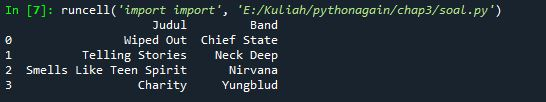
\includegraphics[scale=0.5]{figures/pandasSederhana.JPG}
	\caption{Hasil Pandas Sederhana}
\end{figure}

\item buat aplikasi sederhana menggunakan numpy dan jelaskan arti dari setiap baris kode yang dibuat(harus beda dengan teman sekelas)
\begin{lstlisting}[language=Python]
    #%% 2. Numpy sederhana
    fa = np.array([14,12,20]) # variable fa untuk menampung array 1 dimensi 
    print(fa) #untuk menampilkan hasil variable fa 
\end{lstlisting}
\begin{figure}[!htbp]
    \centering
    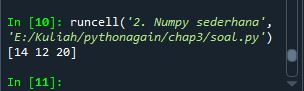
\includegraphics[scale=0.5]{figures/numpySederhana.JPG}
	\caption{Hasil Numpy Sederhana}
\end{figure}

\item buat aplikasi sederhana menggunakan matplotlib dan jelaskan arti dari setiap baris kode(harus beda dengan teman sekelas)
\begin{lstlisting}[language=Python]
    #%% 3. Matplotlib sederhana =  untuk memvisualisasikan data ke dalam bentuk grafik

    x = [1,2,3,5,6,7,3] #variable x untuk menampung semua value dan juga sebagai sumbu x
    y = [1,2,3,3,2,4,5] #variable y untuk menampung semua value dan juga sebagai sumbu y
    
    plt.plot(x, y) #ploting varible x dan y
    
    plt.xlabel('sumbu x') #memberikan label untuk variable x
    plt.ylabel('sumbu y') #memberikan label untuk variabel y
    
    plt.title('Matplotlib sederhana') #memberi title/judul pada plotting yang dibuat
    
    plt.show() #method show digunakan untuk menampilkan plot
\end{lstlisting}
\begin{figure}[!htbp]
    \centering
    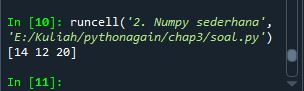
\includegraphics[scale=0.5]{figures/numpySederhana.JPG}
	\caption{Hasil Numpy Sederhana}
\end{figure}

\item jalankan program klasifikasi Random Fores pada bagian teori bab ini. Tunjukkan keluarannya dari komputer sendiri dan artikan maksud setiap luaran yang didapatkan.
\begin{figure}[!htbp]
    \centering
    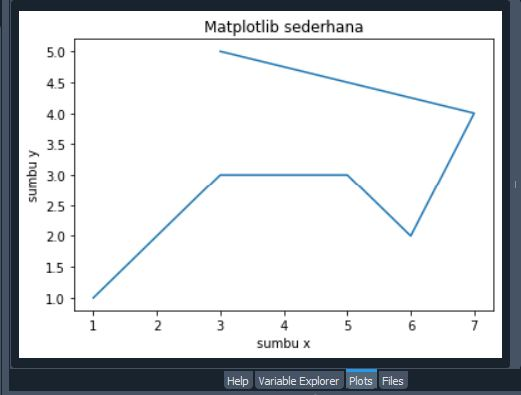
\includegraphics[scale=0.5]{figures/Mtplotlibsederhana.JPG}
	\caption{Hasil Random Forest}
\end{figure}

\newpage
\item jalankan program confusion matrix pada bagian teori bab ini. Tunjukkan keluarannya dari komputer sendiri dan artikan maksud setiap luaran yang didapatkan.
\begin{figure}[!htbp]
    \centering
    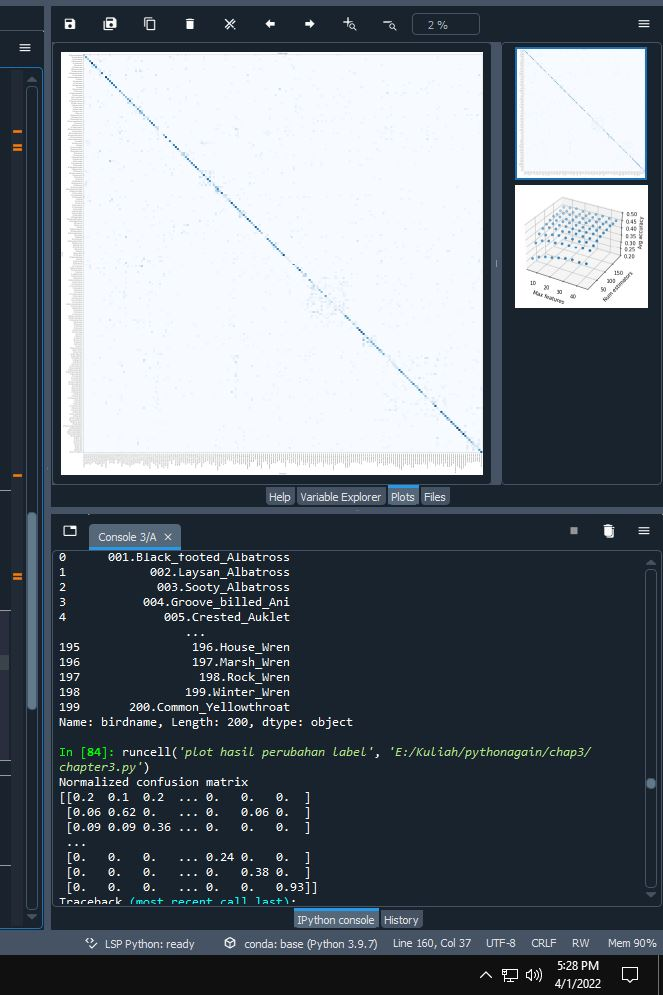
\includegraphics[scale=0.5]{figures/chap3ConfusionMatrix.JPG}
	\caption{Hasil  ConfusionMatrix}
\end{figure}

\newpage
\item jalankan program klasifikasi SVM dan Decission Tree pada bagian teori bab ini. Tunjukkan keluarannya dari komputer sendiri dan artikan maksud setiap luaran yang didapatkan.
\begin{figure}[!htbp]
    \centering
    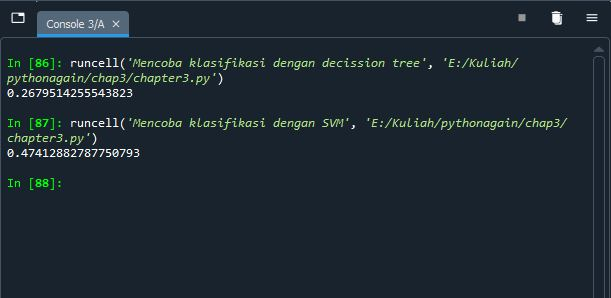
\includegraphics[scale=0.5]{figures/chap3SVMdanDT.JPG}
	\caption{Hasil Klasifikasi DT}
\end{figure}

\item jalankan program cross validaiton pada bagian teori bab ini. Tunjukkan keluarannya dari komputer sendiri dan artikan maksud setiap luaran yang didapatkan.
\newpage
\begin{figure}[!htbp]
    \centering
    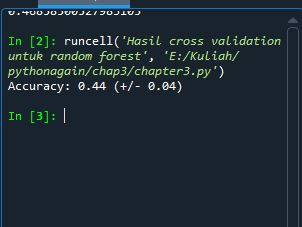
\includegraphics[scale=0.6]{figures/chap3CVjangRF.JPG}
    \caption{Hasil Cross Validation Random Forest}
    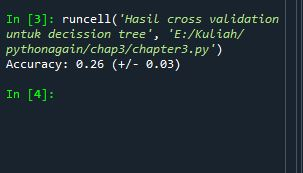
\includegraphics[scale=0.6]{figures/chap3CVjangDT.JPG}
    \caption{Hasil Cross Validation Klasifikasi DT}
    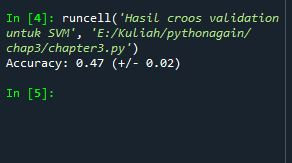
\includegraphics[scale=0.6]{figures/chap3CVjangSVM.JPG}
	\caption{Hasil Cross Validation SVM}
\end{figure}

\item jalankan program pengamatan komponen informasi pada bagian teori bab ini. Tunjukkan keluarannya dari komputer sendiri dan artikan maksud setiap luaran yang didapatkan.
\newpage
\begin{figure}[!htbp]
    \centering
    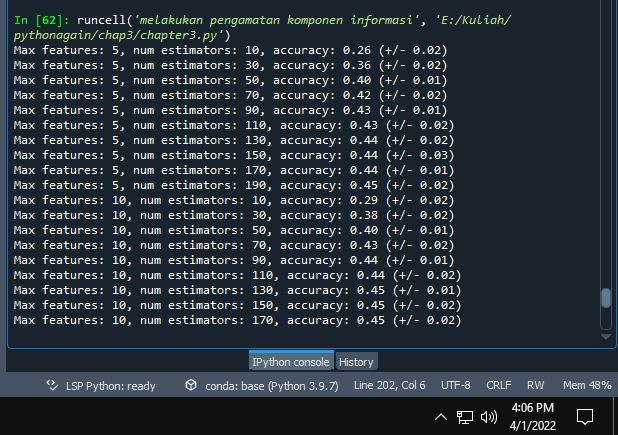
\includegraphics[scale=0.6]{figures/chap3komponeninformasi.JPG}
    \caption{Hasil pengamatan komponen informasi}
    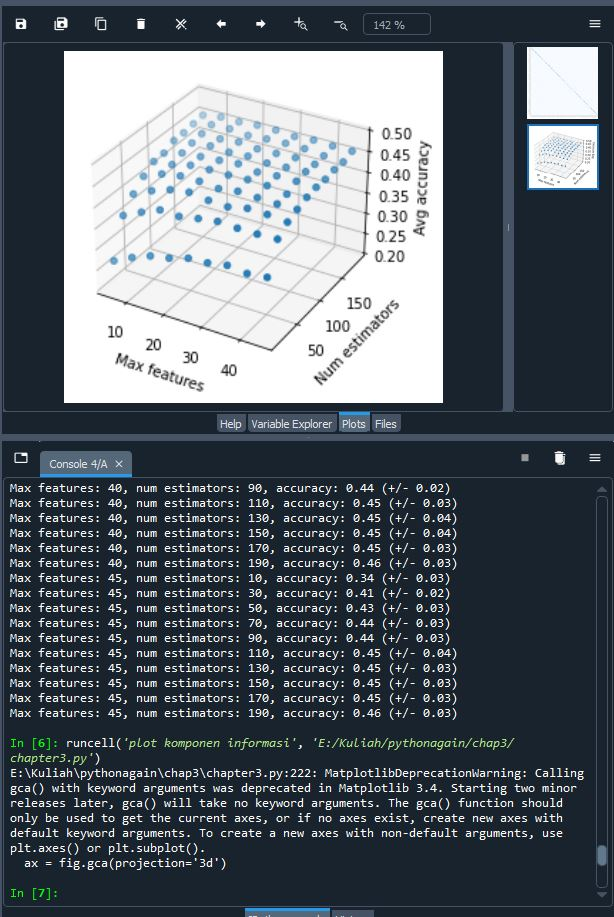
\includegraphics[scale=0.4]{figures/chap3plotkomponen.JPG}
    \caption{Hasil Plot Komponen Informasi}
\end{figure}
\end{enumerate}


\section{Penanganan Error}
Dari percobaan yang dilakukan di atas, error yang kita dapatkan di dokumentasikan dan di selesaikan(nilai 5 per error yang ditangani. Untuk hari kedua):

\begin{enumerate}
	\item skrinsut error
	\item Tuliskan kode eror dan jenis errornya
	\item Solusi pemecahan masalah error tersebut
\end{enumerate}

\section{Presentasi Tugas}
Pada pertemuan ketiga ini, diadakan tiga penilaiain yaitu penilaian untuk tugas mingguan seperti sebelumnya dengan nilai maksimal 100. Kemudian dalam satu minggu kedepan maksimal sebelum waktu mata kuliah kecerdasan buatan. Ada presentasi tugas bab ini dan bab sebelumnya dengan nilai presentasi yang terpisah masing-masing 100. Jadi ada tiga komponen penilaiain pada pertemuan ini yaitu :
\begin{enumerate}
	\item tugas minggu hari ini dan besok (maks 100). pada chapter ini
	\item presentasi decission tree (maks 100). Mempraktekkan kode python dan menjelaskan cara kerjanya.
	\item presentasi Random Forest (maks 100).Mempraktekkan kode python dan menjelaskan cara kerjanya.
\end{enumerate}
Waktu presentasi pada jam kerja di IRC. Kriteria penilaian presentasi sangat sederhana, jika presenter tidak bisa menjawab pertanyaan asisten maka nilai nol. Jika semua pertanyaan bisa dijawab maka nilai 100. Presentasi bisa diulang apabila nilai nol sampai bisa mendapatkan nilai 100 dalam waktu satu minggu kedepan.



% \include{section/chapter4}
% \include{section/chapter5}
% \include{section/chapter6}
% \include{section/chapter7}
% \include{section/chapter8}
% \include{section/chapter9}
% \include{section/chapter10}
% \include{section/chapter11}
% \include{section/chapter12}
% \include{section/chapter13}
% \include{section/chapter14}

%now enable appendix numbering format and include any appendices
% \appendix
% \include{section/appendix1}
% \include{section/appendix2}

% %next line adds the Bibliography to the contents page
% \addcontentsline{toc}{chapter}{Bibliography}
% %uncomment next line to change bibliography name to references
% %\renewcommand{\bibname}{References}
% \bibliography{references}        %use a bibtex bibliography file refs.bib
% \bibliographystyle{plain}  %use the plain bibliography style

\end{document}

